\documentclass[red]{tutorial}
\usepackage[no-math]{fontspec}
\usepackage{xpatch}
	\renewcommand{\ttdefault}{ul9}
	\xpatchcmd{\ttfamily}{\selectfont}{\fontencoding{T1}\selectfont}{}{}
	\DeclareTextCommand{\nobreakspace}{T1}{\leavevmode\nobreak\ }
\usepackage{polyglossia} % English please
	\setdefaultlanguage[variant=us]{english}
%\usepackage[charter,cal=cmcal]{mathdesign} %different font
%\usepackage{avant}
\usepackage{microtype} % Less badboxes

%\usepackage{enumitem}

\usepackage[charter,cal=cmcal]{mathdesign} %different font
%\usepackage{euler}
 
\usepackage{blindtext}
\usepackage{calc, ifthen, xparse, xspace}
\usepackage{makeidx}
\usepackage[hidelinks, urlcolor=blue]{hyperref}   % Internal hyperlinks
\usepackage{mathtools} % replaces amsmath
\usepackage{bbm} %lower case blackboard font
\usepackage{amsthm, bm}
\usepackage{thmtools} % be able to repeat a theorem
\usepackage{thm-restate}
\usepackage{graphicx}
\usepackage[dvipsnames]{xcolor}
\usepackage{multicol}
\usepackage{fnpct} % fancy footnote spacing
\usepackage{tikz}
\usetikzlibrary{arrows.meta}

\usepackage{pgfplots}
\pgfplotsset{compat=1.18}
%\pgfkeys{/pgf/fpu}

 
\newcommand{\xh}{{{\mathbf e}_1}}
\newcommand{\yh}{{{\mathbf e}_2}}
\newcommand{\zh}{{{\mathbf e}_3}}
\newcommand{\R}{\mathbb{R}}
\newcommand{\Z}{\mathbb{Z}}
\newcommand{\N}{\mathbb{N}}
\newcommand{\proj}{\mathrm{proj}}
\newcommand{\Proj}{\mathrm{proj}}
\newcommand{\Perp}{\mathrm{perp}}
\renewcommand{\span}{\mathrm{span}\,}
\newcommand{\Span}{\mathrm{span}\,}
\newcommand{\Img}{\mathrm{img}\,}
\newcommand{\Null}{\mathrm{null}\,}
\newcommand{\Range}{\mathrm{range}\,}
\newcommand{\rref}{\mathrm{rref}}
\newcommand{\rank}{\mathrm{rank}}
\newcommand{\Rank}{\mathrm{rank}}
\newcommand{\nnul}{\mathrm{nullity}}
\newcommand{\mat}[1]{\begin{bmatrix}#1\end{bmatrix}}
\newcommand{\chr}{\mathrm{char}}
\renewcommand{\d}{\mathrm{d}}


\theoremstyle{definition}
\newtheorem{example}{Example}[section]
\newtheorem{defn}{Definition}[section]

%\theoremstyle{theorem}
\newtheorem{thm}{Theorem}[section]

\pgfkeys{/tutorial,
	name={Tutorial 5},
	author={Jason Siefken \& Bernardo Galv\~ao-Sousa},
	course={MAT 244},
	date={},
	term={},
	title={Peer Assisted Reflection}
	}

\begin{document}
	\begin{tutorial}
		\begin{objectives}
	In this tutorial you will MAT 244's expectations around mathematical communication as well
	as what makes a good executive summary.
\end{objectives}

\vspace{-.5em}
\subsection*{Problems}
\vspace{-.5em}

%%%%%%%%%%%%%%%%%%%%%%%%%%

\begin{enumerate}
	\item The first step in solving a mathematics question is applying and understanding logic until \emph{you}
	under the question and its answer. The second step is documenting and communicating your steps/argument. 
	

	Below are questions that might appear on a MAT244 exam paired with possible answers.

	\begin{enumerate}
		\item[(A1)] \emph{Write the complete solution to $y'=2y$. No work necessary.}

		\fbox{
		\begin{minipage}{0.4\textwidth}
			\begin{itemize}
				\item[] $y=Ae^{2t}$
			\end{itemize}
		\end{minipage}
		}

		\item[(A2)] \emph{Let $f$ be a solution to $y'=2y$ satisfying $f(0)=1$. Use Euler's method to approximate $f(2)$. Explain how you arrived at your answer.}
		
		\fbox{
		\begin{minipage}{0.4\textwidth}
			\begin{itemize}
				\item[] $\Delta=0.5$
				\item[] $f_{n+1}=f_{n}+2f_{n}\Delta$
				\item[] $f_0=1$
				\item[] $f(2)\approx 16$
			\end{itemize}
		\end{minipage}
		}

		\item[(A3)] \emph{Let $\vec r\,'(t)=M\vec r(t)$ be a differential equation and let $\vec p(t)$ and $\vec q(t)$
		be solutions. Show that $\vec s = \vec p+\vec q$ is also a solution.}

		
		\fbox{
		\begin{minipage}{0.4\textwidth}
		\begin{itemize}
			\item[] $\vec s\,'=\vec p\,'+\vec q\,'$
			\item[] $\vec p\,'=A\vec p$
			\item[] $\vec q\,'=A\vec q$
			\item[] $\vec p\,'+\vec q\,' = A\vec p+A\vec q$
			\item[] $A(\vec p+\vec q) = A\vec p+A\vec q$
			\item[] $A\vec s=A(\vec p+\vec q)$
			\item[] $\vec s\,'=A\vec s$
		\end{itemize}
		\end{minipage}
		}
		

	\end{enumerate}

	\bigskip
	\begin{enumerate}
		\item Read through each question/answer pair. Are there \emph{logical} errors in the answers? If so, what are they?
		\item On a test, (A1) would be worth 2 points, and (A2) and (A3) would be worth 4 points. How many points do you think
			each answer would be awarded? Why?
		\item The actual scoring for each question was as follows: (A1) 1/2 points, (A2) 0/4 points, and (A3) 1/4 points. What is missing from each
		answer that is prevent it from getting full marks?
		\item Fix each argument so that it would receive full marks.
	\end{enumerate}

	\item As part of your final report and your Homework 3, you will be writing an executive summary. The University of Southern California (USC)
	provides guidelines for what makes a good executive summary at \url{https://libguides.usc.edu/writingguide/executivesummary}
	
	Recall the \emph{bee} question from Homework 2. Imagine that you were commissioned by a farmer to study bees in his field and
	to give him guidance on where to plant his flowers so that they will be pollinated.

			\vspace{-.3cm}
	\begin{enumerate}
		\item Read through the USC guidelines. What are three things you would expect to appear in an executive summary for the bee question?
		\item The following is an executive summary for the bee question created by an AI. 

		\framebox{
		\begin{minipage}{0.8\textwidth}
			\small The summary of the bee's behavior can be described as
			follows:

			\vspace{-.3cm}
			\paragraph{In English:}

			The bee's movement is modeled based on the intensity of flower smell and its
			distance from the hive. The bee travels in a field of flowers, where the smell
			intensity varies on a logarithmic scale. The bee's movement is influenced
			by both the current smell intensity and its distance from the hive. The model
			suggests that bees will only stay still in the hive or on a flower, and
			flowers are located at specific distances from the hive. The bee's behavior
			includes moving towards or away from the hive based on smell intensity,
			potentially overshooting its target before settling on a flower. Odd-numbered
			flowers tend to attract bees, while even-numbered flowers are unstable
			points.

			\vspace{-.3cm}
			\paragraph{In mathematical terms:}
			\[
				\begin{cases}
					S'(t) & = \sin(D(t))   \\
					D'(t) & = S(t) - D(t)
				\end{cases}
			\]
			Where:
			\begin{itemize}
				\item $S(t) =$ intensity of flower smell at time $t$ (logarithmic scale
					from $-\infty$ to $+\infty$)

				\item $D(t) =$ (positive) distance between the bee and its hive at time $t$
			\end{itemize}

			\vspace{-.3cm}
			\paragraph{Key points:}

			Smell intensity is constant when $S' = 0$, which occurs when $\sin(D) = 0$
			or $D = n\pi$, where $n$ is a non-negative integer.

			Flowers are located at distances $k\pi$ from the hive, where $k > 0$ is a
			whole number.

			The system can be simulated using Euler's method for the differential
			equations.

			Phase portraits show that odd-numbered flowers are attracting points, while
			even-numbered ones are unstable.

			There's a critical smell intensity (around 7.1 $\pm$ 0.01) that determines
			whether a bee will fly to the 1st or 3rd flower when starting from the hive.

			\medskip
			This model captures the essence of how bees navigate using smell intensity
			and distance from their hive to locate flowers in a field.
		\end{minipage}
		}

		\begin{enumerate}
			\item What did the AI do well in the executive summary?
			\item What did the AI do poorly?
			\item Executive summaries rarely include mathematical formulas. Do you agree with its choice to include one? What is the alternative?
			\item The AI's executive summary does not directly address the farmer's question about where to plant flowers.

			Write an introductory paragraph to a new executive summary that addresses the farmer's question.
		\end{enumerate}

		\item For Homework 3, you are asked to write an executive summary. What key items should your executive summary for Homework 3 include?
		What would be a good introductory paragraph?

	\end{enumerate}


	%\item We gave the AI$^{0}$ the Executive Summary guidelines from the
	%	University of Southern California. Below is the revised Executive Summary.

	%	\hspace{-1cm}
	%	\framebox{
	%	\begin{minipage}{\textwidth}
	%		\small
	%		\paragraph{Executive Summary:}
	%		Bee Behavior Model Analysis\\

	%		This study examines a mathematical model of bee behavior in a field of
	%		flowers, focusing on the relationship between smell intensity and the bee's
	%		distance from its hive. The model uses differential equations to describe
	%		the bee's movement and decision-making process. \\

	%		\paragraph{Key Findings:}
	%		Smell intensity is constant at specific distances from the hive,
	%		particularly when the distance is a non-negative multiple of $\pi$.

	%		Flowers are located at distances that are multiples of $\pi$ from the hive.

	%		When a bee starts at a distance of 5 units from its hive with neutral
	%		smell intensity, it initially moves towards the hive, then towards the
	%		first flower, eventually settling on the flower at a distance of $\pi$ from
	%		the hive.

	%		Odd-numbered flowers (at distances $\pi, 3\pi, 5\pi$, etc.) attract bees,
	%		while even-numbered flowers are unstable attractors.

	%		The minimum smell intensity required for a bee to venture to the third
	%		flower ($3\pi$ distance) from its hive is approximately $7.1 \pm 0.01$ on
	%		the logarithmic scale used in the model. \\

	%		\paragraph{Methodology:}
	%		The study employed a mix of analytic arguments, computer-based simulations
	%		using Euler's method, and qualitative analysis techniques such as phase portraits.

	%		\paragraph{Implications:}
	%		This model provides insights into bee foraging behavior, suggesting that bees
	%		are more likely to visit certain flowers based on their distance from the hive
	%		and the intensity of their smell. This information could be valuable for
	%		understanding pollination patterns and optimizing flower placement in
	%		agricultural settings. \\

	%		\paragraph{Recommendations:}
	%		Further research to validate the model's predictions in real-world scenarios.
	%		Exploration of how environmental factors might influence the model's
	%		parameters. Investigation of potential applications in agriculture and ecology.
	%		\\

	%		This executive summary provides a concise overview of the bee behavior model,
	%		its key findings, and potential implications, serving as a foundation for
	%		further discussion and research in this area.
	%	\end{minipage}
	%	}

\end{enumerate}

%%%%%%%%%%%%%%%%%%%%%%%%%%
	\end{tutorial}

	\begin{solutions}
		
	
\begin{enumerate}
    \item \begin{enumerate}
        \item Though we cannot know exactly what the author of each answer was thinking, the steps do not appear to have logical contradictions.
        \item 
        \item Question (A1) has no explanation of what $A$ is (or $t$ for that matter). Neither (A2) nor (A3) have any words at all.
        They should be written in complete (mathematical) sentences.
        \item 

        \begin{enumerate}
            \item[(A1)] \emph{Write the complete solution to $y'=2y$. No work necessary.}

            \fbox{
            \begin{minipage}{0.78\textwidth}
                \begin{itemize}
                    \item[] $y=Ae^{2t}$ where $A\in\R$ is a parameter.
                \end{itemize}
            \end{minipage}
            }

            \item[(A2)] \emph{Let $f$ be a solution to $y'=2y$ satisfying $f(0)=1$. Use Euler's method to approximate $f(2)$. Explain how you arrived at your answer.}
            
            \fbox{
            \begin{minipage}{0.78\textwidth}
                \begin{itemize}
                    \item[] We will use a step size of $\Delta=0.5$.
                    \item[] Let $f_n$ be the approximation we get from the $n$th application of Euler's method. 
                    Since $f'=2f$, using a tangent line approximation, we get the recursive formula
                    \[
                        f_{n+1}=f_{n}+2f_{n}\Delta
                    \]
                    \item[] We start with initial condition $f(0)=1$. I.e., $f_0=1$.
                    \item[] After iterating four times, we get \[f(2)\approx 16.\]
                \end{itemize}
            \end{minipage}
            }

            \item[(A3)] \emph{Let $\vec r\,'(t)=M\vec r(t)$ be a differential equation and let $\vec p(t)$ and $\vec q(t)$
            be solutions. Show that $\vec s = \vec p+\vec q$ is also a solution.}

            
            \fbox{
            \begin{minipage}{0.78\textwidth}
            \begin{itemize}
                \item[] Because the derivative is linear, we have $\vec s\,'=\vec p\,'+\vec q\,'$.
                \item[] Note that $\vec p\,'=A\vec p$,
                \item[] and $\vec q\,'=A\vec q$.
                \item[] Thus, $\vec p\,'+\vec q\,' = A\vec p+A\vec q$.
                \item[] Because matrix multiplication is also linear, we have the identity $A(\vec p+\vec q) = A\vec p+A\vec q$.
                \item[] Combining this with our previous formula, we see $A\vec s=A(\vec p+\vec q)$,
                \item[] and so $\vec s\,'=A\vec s$, which means $\vec s$ is a solution to the differential equation.
            \end{itemize}
            \end{minipage}
            }
        \end{enumerate}
    \end{enumerate}

        \item \begin{enumerate}
            \item I would expect an opening statement explaining how bees can only pollinate flowers they can land on,
            an overview of the model stating that it was based on differential equations and simulated using Euler's method,
            and a summary of the model's results about how bees can only land on ``odd numbered'' flowers.

            \item \begin{enumerate}
                \item The AI wrote in complete sentences. It split the summary into sections with headings, and it 
                provided a summary of the results of the model.
                \item The AI did not explain how the model is relevant to the farmer's question about where to plant flowers.
                It used overly-technical equations, and is overall written in a boring style that does not encourage the reader to continue.
                \item No, the formulas included, while the basis for the model, are not self-explanatory. It takes simulations and phase 
                portraits to understand what is going on and so including the formulas in the executive summary is not helpful. Instead,
                the formulas belong in the body of the report. The executive summary itself should be more high-level, including things like
                ``a system of differential equations was used to model the bees; it was simulated using Euler's method\ldots''.

                \item \phantom{x}\begin{quote}
                    Bees are the primary pollinator of <your crop> and as common sense suggests, bees will only pollinate flowers
                    that they can land on. This report shows gives the details of a differential-equations based model predicting
                    that if you place a hive, flowers that grow at distances approximately $3.1$, $9.2$, $12.4$ metres away from the hive
                    will attract bees while other flowers will not. The findings suggest that you should follow specific planting patterns
                    to maximize pollination.
                \end{quote}
            \end{enumerate}
        \item
        \end{enumerate}
		

\end{enumerate}
	
	\end{solutions}
	\begin{instructions}
		\subsection*{Learning Objectives}
	Students need to be able to\ldots
	\begin{itemize}
		\item recognize and provide good feedback using the SPARK guidelines.	\end{itemize}

\subsection*{Context}
	This week, students will be providing feedback on their peers' modelling for Homework \#3. As such, there are no problems for students to solve in tutorial.
	

\subsection*{Before Tutorial}

Send an announcement reminding students that they need to bring a draft of Q4 for homework \#3.

\subsection*{What to Do}

	\paragraph{How to provide good feedback (15-20 min)}

	SPARK guidelines.
	
	Essentially, you will be replicating the workshop done in the head TA meetings this week.
	
	Start by asking students what they think makes a piece of feedback good or bad. They can either explain, or give examples. Connect these examples to the SPARK guidelines to explain what makes this feedback good or bad.
	
	If students don't provide any convenient examples, here are the examples of good/bad feedback we saw in this week's workshop:
	\begin{itemize}
		\item ``Everything is perfect!''
		\item ``Your grammar sucks. Did you even use spellcheck?!''
		\item ``You should delete parts of this section from your modelling, you don't need them.''
%		\item ``Your mind map has too many concepts in it. These are good ideas, but the mindmap should be readable without zooming in. I think you should remove at least five of them.''
		\item ``This sentence is very long, which makes it hard to read; you could split it into 3 sentences if you put periods in these places. If you need extra help with writing, your college probably has a writing centre you can use.''
		\item ``I thought it was insightful that you discussed the decline of the lobster fishing industry in your hometown as a reason for exponential population decrease. You've clearly shown your knowledge of your hometown's culture and how it affects the population in mathematical terms.''
	\end{itemize}
	
	The SPARK guidelines are as follows:
	\begin{itemize}
		\item \textbf{Specific:} Comments are linked to a discrete word, phrase, or sentence.
		\item \textbf{Prescriptive:} Prescriptive feedback offers a solution or strategy to improve the work, including possible revisions or links to helpful resources or examples.
		\item \textbf{Actionable:} When the feedback is read, it leaves the peer knowing what steps to take for improvement.
		\item \textbf{Referenced:} The feedback directly references the task criteria, requirements, or target skills.
		\item \textbf{Kind:} It's mandatory that all comments be framed in a kind, supportive way.
	\end{itemize}
	
	

\subsection*{Notes}
	\begin{itemize}
		\item Feedback doesn't need to be critical to be good; positive feedback can also be useful in telling students what to continue doing, as long as it still embodies the SPARK guidelines.
		\item Encourage students to review the feedback that is given to them. If students don't feel that the feedback they receive is useful, they should ask their partner to elaborate.

\end{itemize}
	
	

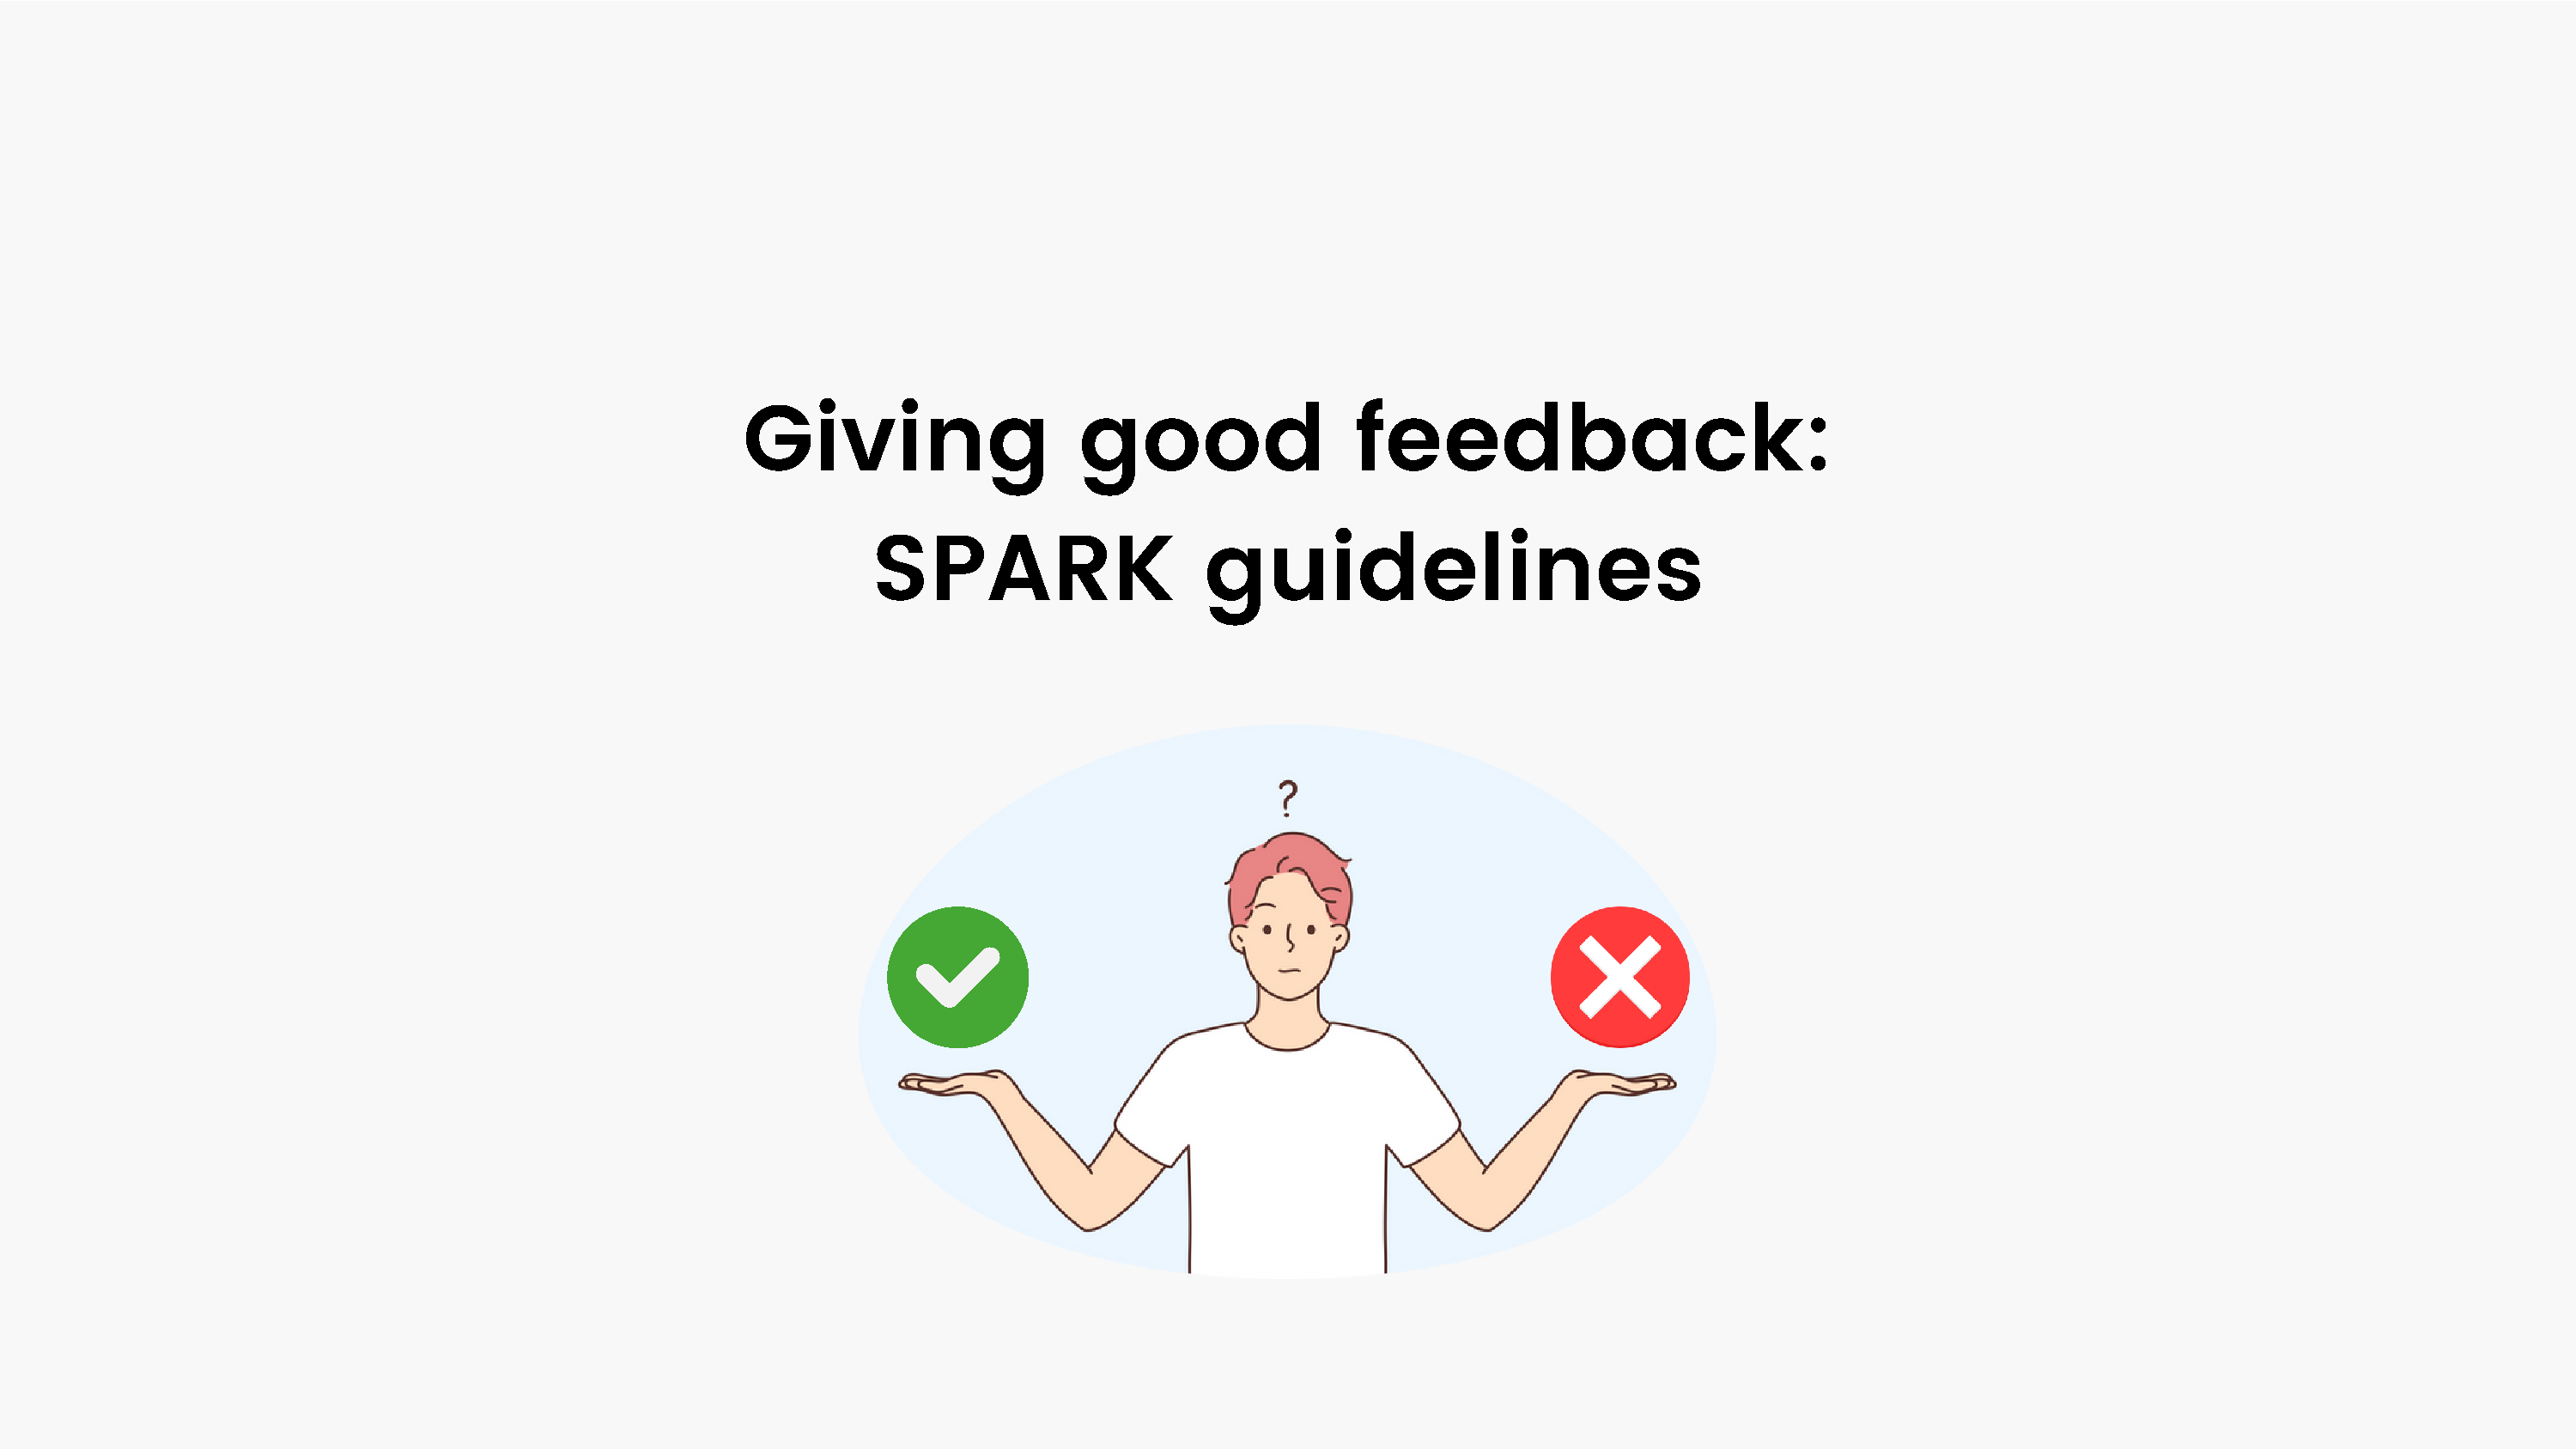
\includegraphics[page=1,width=\textwidth]{resources/tutorial-05-WorkshopFeedbackSPARK.pdf}
\vfil
\includegraphics[page=2,width=\textwidth]{resources/tutorial-05-WorkshopFeedbackSPARK.pdf}
\vfil
\includegraphics[page=3,width=\textwidth]{resources/tutorial-05-WorkshopFeedbackSPARK.pdf}
\vfil
\includegraphics[page=4,width=\textwidth]{resources/tutorial-05-WorkshopFeedbackSPARK.pdf}
\vfil
\includegraphics[page=5,width=\textwidth]{resources/tutorial-05-WorkshopFeedbackSPARK.pdf}
\vfil
\includegraphics[page=6,width=\textwidth]{resources/tutorial-05-WorkshopFeedbackSPARK.pdf}
\vfil
\includegraphics[page=7,width=\textwidth]{resources/tutorial-05-WorkshopFeedbackSPARK.pdf}
\vfil
\includegraphics[page=8,width=\textwidth]{resources/tutorial-05-WorkshopFeedbackSPARK.pdf}


	
	

	\end{instructions}

\end{document}
